\documentclass[varwidth,border=0pt]{standalone}

% Tikz packages
\usepackage{tikz}
\usetikzlibrary{%
  patterns, plotmarks, backgrounds, shapes, arrows, calc, trees, positioning,
  chains, shapes.geometric, decorations.pathreplacing,
  decorations.pathmorphing, shapes.arrows, decorations.markings, quotes,
  arrows.meta, spy, fit, matrix
}
\tikzset{%
  hexagon/.style={signal,signal to=east and west}
}

% General image and colour support
\usepackage{graphicx}
\usepackage{xcolor}

% Captions and subcaptions
\usepackage{caption}
\usepackage[labelformat=parens]{subcaption}
\renewcommand\thesubfigure{\alph{subfigure})}

% String macros (for reading in tabular data)
\usepackage{xstring}

%% Define node types
\tikzstyle{lnode} = [%
  circle,
  draw=black,
  minimum height=0.65cm,
  align=center,
  fill=none,
  text centered,
  inner sep=0.5pt,
  font=\tiny
]%
\tikzstyle{rx1} = [%
  circle,
  draw=black,
  minimum height=0.10cm,
  align=center,
  fill=none,
  text centered,
  inner sep=0.5pt,
  font=\tiny
]%
\tikzstyle{rx2} = [%
  circle,
  draw=black,
  minimum height=0.20cm,
  anchor=center,
  align=center,
  fill=white,
  text centered,
  inner sep=0.5pt,
  font=\tiny
]%
\tikzstyle{met} = [%
  rectangle,
  rounded corners=3pt,
  draw=black,
  minimum height=0.5cm,
  minimum width=1.0cm,
  align=center,
  fill=none,
  text centered,
  inner sep=0.5pt,
  font=\tiny
]%
\tikzstyle{enz} = [%
  hexagon,
  draw=black,
  minimum height=0.5cm,
  minimum width=0.75cm,
  align=center,
  fill=none,
  text centered,
  inner sep=0.0pt,
  font=\tiny
]

\begin{document}
  \begin{figure}
    \centering
    \begin{subfigure}{1.0\textwidth}
      \scalebox{0.35}{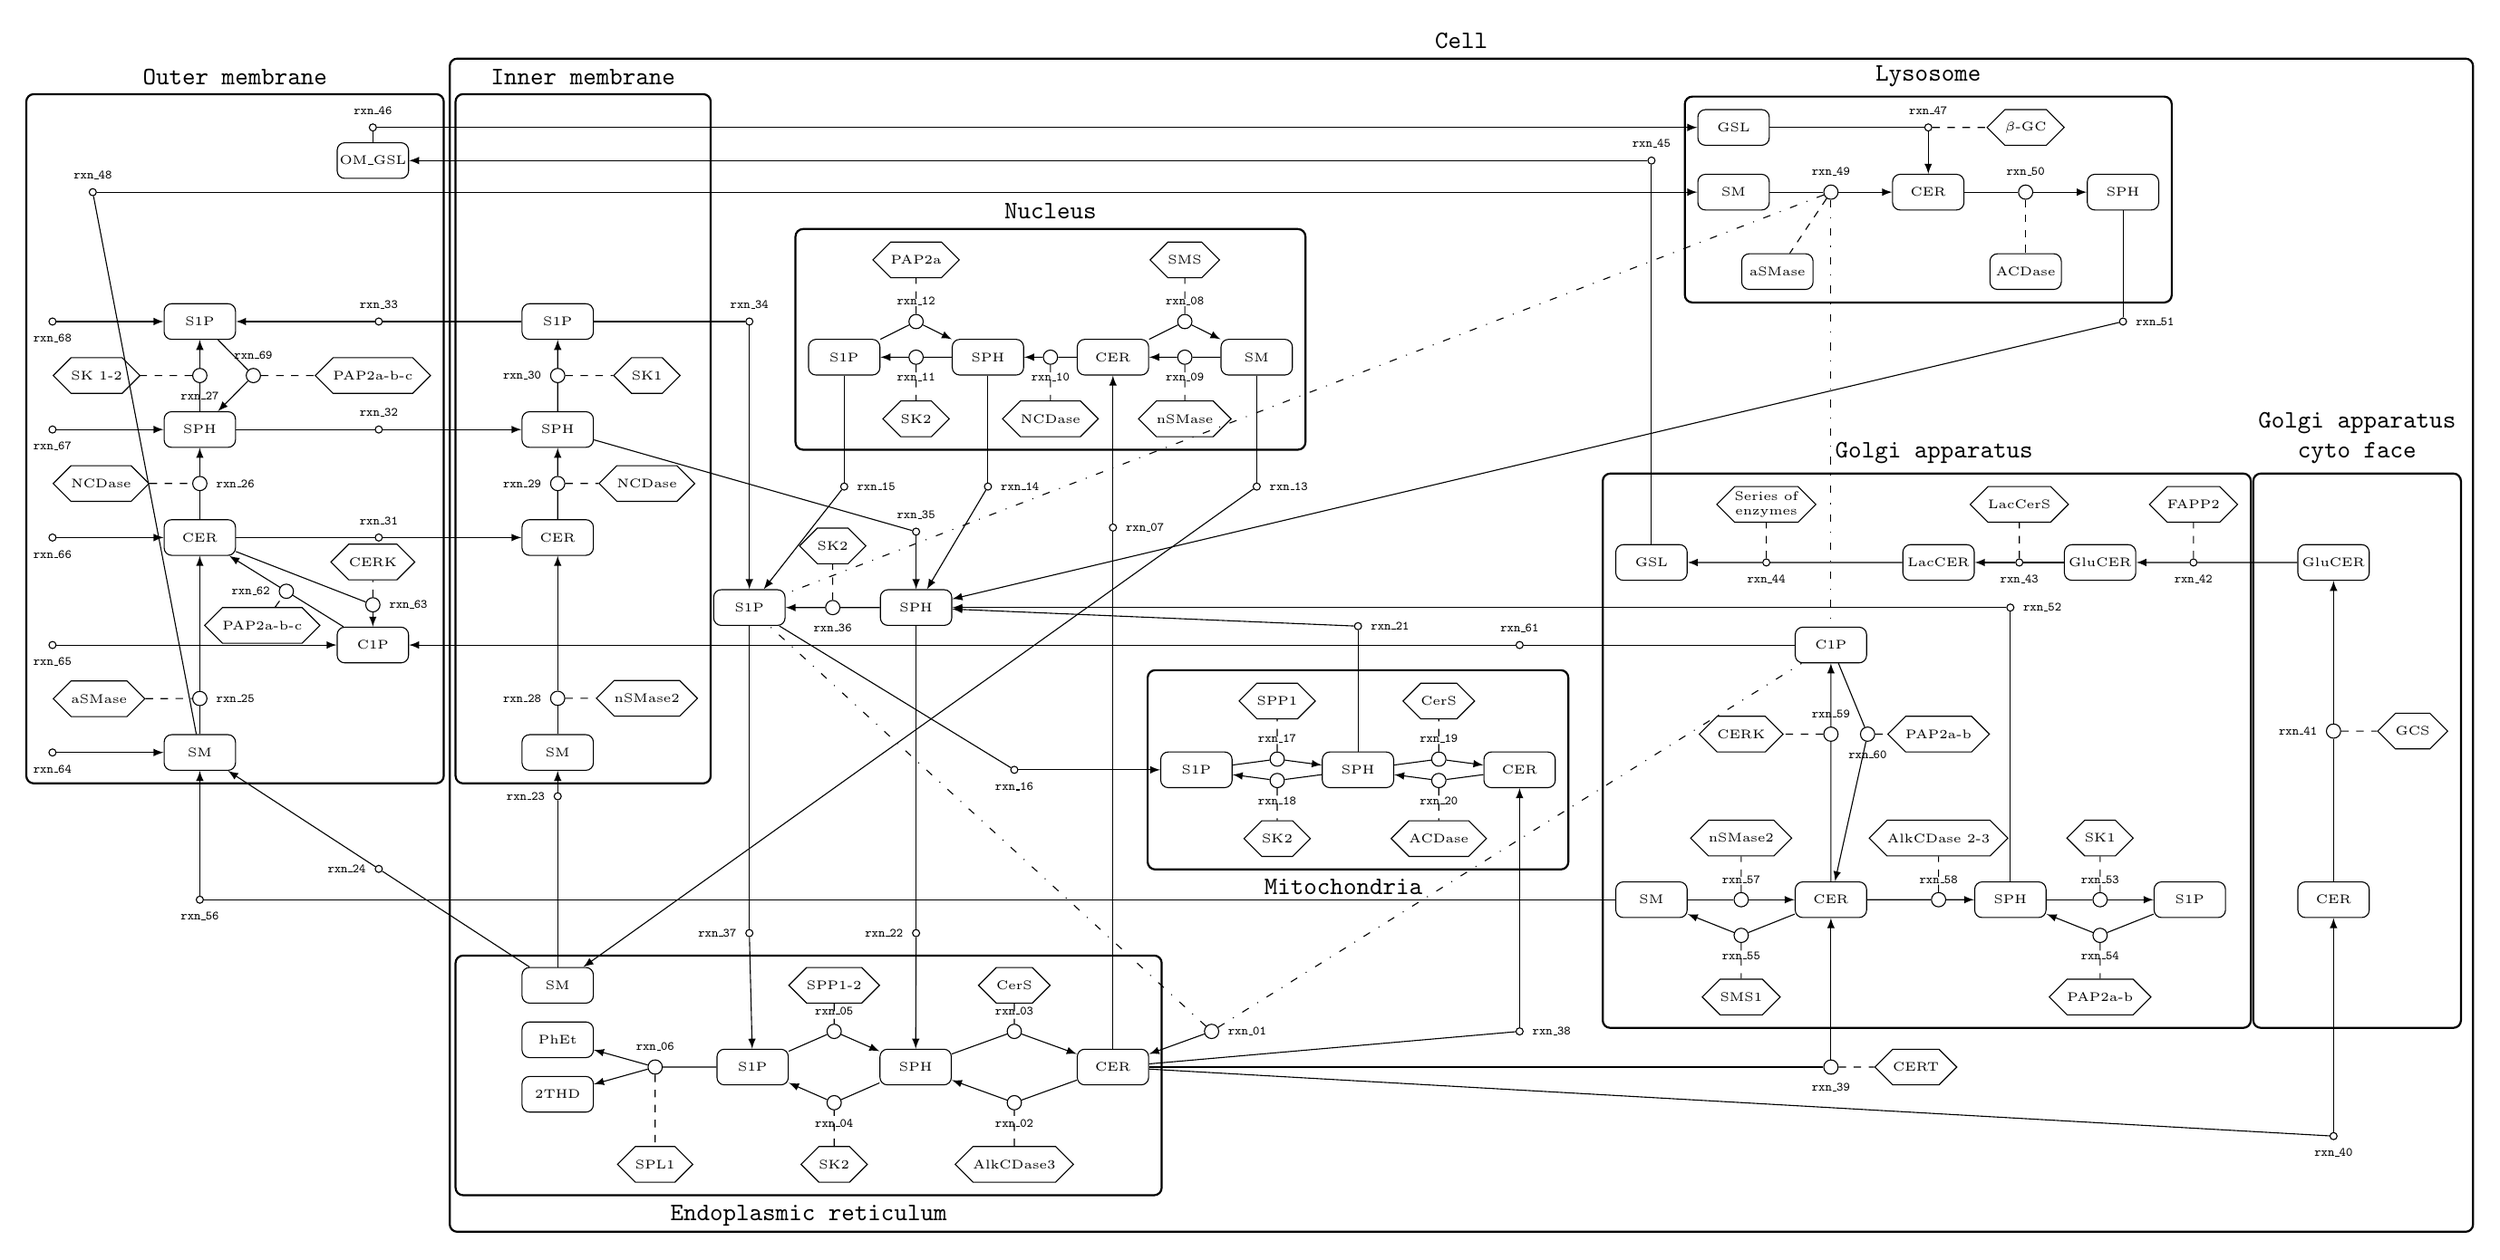
\begin{tikzpicture}[%
  >=latex,
  every node/.style={%
    font=\sffamily\footnotesize\itshape,
    text=black,
    text centered,
    align=center
  },
  frame/.style={%
    draw=black,
    inner sep=2pt
  },
  every label/.style={%
    text=black,
    font=\tiny\ttfamily
  }
]

  % OM nodes (metabolites and some rxn nodes)
  \node[met] (OM_S1P) {S1P};
  \node[rx1,left=1.5cm of OM_S1P, label=below:rxn\_68] (rxn_68) {};
  \node[met,below=1.0cm of OM_S1P] (OM_SPH) {SPH};
  \node[rx2,label=below:rxn\_27] at ($(OM_S1P)!0.5!(OM_SPH)$) (rxn_27) {};
  \node[rx1,left=1.5cm of OM_SPH, label=below:rxn\_67] (rxn_67) {};
  \node[enz,anchor=west] at ($(rxn_67)!0.5!(rxn_68)$) (OM_SK12) {SK 1-2};
  \node[met,below=1.0cm of OM_SPH] (OM_CER) {CER};
  \node[rx1,left=1.5cm of OM_CER, label=below:rxn\_66] (rxn_66) {};
  \node[met,below=2.5cm of OM_CER] (OM_SM) {SM};
  \node[rx1,left=1.5cm of OM_SM, label=below:rxn\_64] (rxn_64) {};
  \node[enz,anchor=west] at ($(rxn_67)!0.5!(rxn_66)$) (OM_NCDASE) {NCDase};
  \node[rx2,xshift=0.75cm,label=above:rxn\_69] at ($(OM_S1P)!0.5!(OM_SPH)$) (rxn_69) {};
  \node[enz,right=0.75cm of rxn_69] (OM_PAP) {PAP2a-b-c};
  \node[enz,anchor=west] at ($(rxn_64)!0.25!(rxn_66)$) (OM_aSMase) {aSMase};
  \node[rx1,below=1.75cm of OM_SM, label=below:rxn\_56] (rxn_56) {};
  \node[met,above=2.5cm of OM_PAP] (OM_GSL) {OM\_GSL};
  \node[rx1,above=0.15cm of OM_GSL, label=above:rxn\_46] (rxn_46) {};
  \node[rx1,label=below:rxn\_65] at ($(rxn_64)!0.5!(rxn_66)$) (rxn_65) {};
  \node[met] at (rxn_65 -| OM_PAP) (OM_C1P) {C1P};
  \node[enz,left=0.225cm of OM_C1P,yshift=0.275cm] (OM_PAP2) {PAP2a-b-c};
  \node[enz,above=0.65cm of OM_C1P] (OM_CERK) {CERK};
  \node[rx2,above=0.2cm of OM_C1P,label=right:rxn\_63] (rxn_63) {};
  \node[rx1,above=1.5cm of OM_S1P,xshift=-1.5cm,label=above:rxn\_48] (rxn_48) {};

  % IM nodes (metabolites and some rxn nodes)
  \node[met,right=4.0cm of OM_S1P] (IM_S1P) {S1P};
  \node[met,below=1.0cm of IM_S1P] (IM_SPH) {SPH};
  \node[met,below=1.0cm of IM_SPH] (IM_CER) {CER};
  \node[met,below=2.5cm of IM_CER] (IM_SM) {SM};
  \node[rx2,label=left:rxn\_30] at ($(IM_S1P)!0.5!(IM_SPH)$) (rxn_30) {};
  \node[enz,xshift=1.25cm] at ($(IM_S1P)!0.5!(IM_SPH)$) (IM_SK1) {SK1};
  \node[rx2,label=left:rxn\_29] at ($(IM_CER)!0.5!(IM_SPH)$) (rxn_29) {};
  \node[enz,xshift=1.25cm] at ($(IM_CER)!0.5!(IM_SPH)$) (IM_NCDase) {NCDase};
  \node[rx2,above=0.396cm of IM_SM,label=left:rxn\_28] (rxn_28) {};
  \node[enz,anchor=center] at (rxn_28 -| IM_NCDase) (IM_nSMase2) {nSMase2};
  \node[rx1,below=0.30cm of IM_SM, label=left:rxn\_23] (rxn_23) {};

  % ER nodes (metabolites and some rxn nodes)
  \node[met,below=2.75cm of IM_SM,fill=white] (ER_SM) {SM};
  \node[met,below=0.25cm of ER_SM] (ER_PhEt) {PhEt};
  \node[met,below=0.25cm of ER_PhEt] (ER_2THD) {2THD};
  \node[] at ($(ER_PhEt)!0.5!(ER_2THD)$) (ER_PH) {};
  \node[met,right=2.1cm of ER_PH] (ER_S1P) {S1P};
  \node[met,right=1.27cm of ER_S1P] (ER_SPH) {SPH};
  \node[met,right=1.75cm of ER_SPH] (ER_CER) {CER};
  \node[met,right=1.75cm of ER_CER,draw=white] (ER_PH2) {};
  \node[rx2,label=above:rxn\_06] at ($(ER_PH)!0.5!(ER_S1P)$) (rxn_06) {};
  \node[enz,below=1.0cm of rxn_06] (ER_SPL1) {SPL1};
  \node[rx2,label=above:rxn\_05,yshift=+0.5cm] at ($(ER_S1P)!0.5!(ER_SPH)$) (rxn_05) {};
  \node[rx2,label=below:rxn\_04,yshift=-0.5cm] at ($(ER_S1P)!0.5!(ER_SPH)$) (rxn_04) {};
  \node[rx2,label=above:rxn\_03,yshift=+0.5cm] at ($(ER_CER)!0.5!(ER_SPH)$) (rxn_03) {};
  \node[rx2,label=below:rxn\_02,yshift=-0.5cm] at ($(ER_CER)!0.5!(ER_SPH)$) (rxn_02) {};
  \node[rx2,label=right:rxn\_01,yshift=+0.5cm] at ($(ER_CER)!0.5!(ER_PH2)$) (rxn_01) {};
  \node[enz,anchor=center] at (ER_SM -| rxn_05) (ER_SPP12) {SPP1-2};
  \node[enz,anchor=center] at (ER_SM -| rxn_03) (ER_CerS) {CerS};
  \node[enz,anchor=center] at (ER_SPL1 -| rxn_04) (ER_SK2) {SK2};
  \node[enz,anchor=center] at (ER_SPL1 -| rxn_02) (ER_AlkCDase3) {AlkCDase3};

  % N nodes (metabolites and some rxn nodes)
  \node[met,right=3.0cm of IM_S1P,yshift=-0.5cm] (N_S1P) {S1P};
  \node[met,right=1.0cm of N_S1P] (N_SPH) {SPH};
  \node[met] at (N_SPH -| ER_CER) (N_CER) {CER};
  \node[met,right=1.0cm of N_CER] (N_SM) {SM};
  \node[rx2,label=above:rxn\_12,yshift=+0.5cm] at ($(N_S1P)!0.5!(N_SPH)$) (rxn_12) {};
  \node[rx2,label=below:rxn\_11,yshift=-0.0cm] at ($(N_S1P)!0.5!(N_SPH)$) (rxn_11) {};
  \node[rx2,label=below:rxn\_10,yshift=-0.0cm] at ($(N_SPH)!0.5!(N_CER)$) (rxn_10) {};
  \node[rx2,label=below:rxn\_09,yshift=-0.0cm] at ($(N_CER)!0.5!(N_SM)$) (rxn_09) {};
  \node[rx2,label=above:rxn\_08,yshift=+0.5cm] at ($(N_CER)!0.5!(N_SM)$) (rxn_08) {};
  \node[enz,below=0.5cm of rxn_11] (N_SK2) {SK2};
  \node[enz,above=0.5cm of rxn_12] (N_PAP2a) {PAP2a};
  \node[enz,below=0.5cm of rxn_10] (N_NCDase) {NCDase};
  \node[enz,below=0.5cm of rxn_09] (N_nSMase) {nSMase};
  \node[enz,above=0.5cm of rxn_08] (N_SMS) {SMS};
  \node[rx1,below=1.5cm of N_S1P,label=right:rxn\_15] (rxn_15) {};
  \node[rx1,label=right:rxn\_14] at (rxn_15 -| N_SPH) (rxn_14) {};
  \node[rx1,label=right:rxn\_13] at (rxn_15 -| N_SM) (rxn_13) {};

  % L nodes (metabolites and some rxn nodes)
  \node[met,right=18.5cm of rxn_46] (L_GSL) {GSL};
  \node[met] at (L_GSL |- rxn_48) (L_SM) {SM};
  \node[rx2,right=0.75cm of L_SM,label=above:rxn\_49] (rxn_49) {};
  \node[met,right=0.75cm of rxn_49] (L_CER) {CER};
  \node[rx2,right=0.75cm of L_CER,label=above:rxn\_50] (rxn_50) {};
  \node[met,right=0.75cm of rxn_50] (L_SPH) {SPH};
  \node[rx1,label=above:rxn\_47] at (L_GSL -| L_CER) (rxn_47) {};
  \node[enz] at (rxn_47 -| rxn_50) (L_bGC) {$\beta$-GC};
  \node[met,below=0.75cm of rxn_50] (L_ACDase) {ACDase};
  \node[met,below=0.75cm of rxn_49,xshift=-0.75cm] (L_aSMase) {aSMase};
  \node[rx1,below=1.5cm of L_SPH,label=right:rxn\_51] (rxn_51) {};

  % GA nodes (metabolites and some rxn nodes)
  \node[met] at (OM_C1P -| rxn_49) (GA_C1P) {C1P};
  \node[met] at (rxn_56 -| GA_C1P) (GA_CER) {CER};
  \node[met,left=1.5cm of GA_CER] (GA_SM) {SM};
  \node[rx2,label=above:rxn\_57,yshift=+0.0cm] at ($(GA_SM)!0.5!(GA_CER)$) (rxn_57) {};
  \node[rx2,label=below:rxn\_55,yshift=-0.5cm] at ($(GA_SM)!0.5!(GA_CER)$) (rxn_55) {};
  \node[enz,below=0.5cm of rxn_55] (GA_SMS1) {SMS1};
  \node[met,right=1.5cm of GA_CER] (GA_SPH) {SPH};
  \node[met,right=1.5cm of GA_SPH] (GA_S1P) {S1P};
  \node[rx2,label=above:rxn\_58,yshift=+0.0cm] at ($(GA_CER)!0.6!(GA_SPH)$) (rxn_58) {};
  \node[rx2,label=above:rxn\_53,yshift=+0.0cm] at ($(GA_S1P)!0.5!(GA_SPH)$) (rxn_53) {};
  \node[enz,above=0.5cm of rxn_53] (GA_SK1) {SK1};
  \node[enz] at (GA_SMS1 -| rxn_53) (GA_PAP) {PAP2a-b};
  \node[rx2,label=below:rxn\_54] at (rxn_55 -| rxn_53) (rxn_54) {};
  \node[rx2,label=above:rxn\_59] at ($(GA_C1P)!0.35!(GA_CER)$) (rxn_59) {};
  \node[rx2,label=below:rxn\_60,right=0.3cm of rxn_59] (rxn_60) {};
  \node[enz] at (rxn_59 -| rxn_58) (GA_PAP2) {PAP2a-b};
  \node[enz] at (rxn_57 |- rxn_59) (GA_CERK) {CERK};
  \node[enz,above=0.5cm of rxn_58] (GA_Alk) {AlkCDase 2-3};
  \node[enz,above=0.5cm of rxn_57] (GA_nSMase2) {nSMase2};

  % GACF and upper row GA nodes (metabolites and some rxn nodes)
  \node[met,right=1.0cm of GA_S1P] (GACF_CER) {CER};
  \node[rx2,above=2.0cm of GACF_CER,label=left:rxn\_41] (rxn_41) {};
  \node[met,above=2.0cm of rxn_41] (GACF_GluCER) {GluCER};
  \node[enz,right=0.5cm of rxn_41] (GACF_GCS) {GCS};
  \node[met] at (GA_SK1 |- GACF_GluCER) (GA_GluCER) {GluCER};
  \node[met] at (GA_Alk |- GA_GluCER) (GA_LacCER) {LacCER};
  \node[met] at (GA_SM |- GA_LacCER) (GA_GSL) {GSL};
  \node[rx1,label=below:rxn\_42] at ($(GA_GluCER)!0.4!(GACF_GluCER)$) (rxn_42) {};
  \node[enz,above=0.5cm of rxn_42] (GA_FAPP2) {FAPP2};
  \node[rx1,label=below:rxn\_43] at ($(GA_GluCER)!0.5!(GA_LacCER)$) (rxn_43) {};
  \node[enz,above=0.5cm of rxn_43] (GA_LacCerS) {LacCerS};
  \node[rx1,label=below:rxn\_44] at ($(GA_GSL)!0.4!(GA_LacCER)$) (rxn_44) {};
  \node[enz,above=0.5cm of rxn_44] (GA_Series) {Series of\\enzymes};

  % M nodes (metabolites and some rxn nodes)
  \node[met,left=2.0cm of GA_CERK,yshift=-0.5cm] (M_CER) {CER};
  \node[met,left=1.25cm of M_CER] (M_SPH) {SPH};
  \node[met,left=1.25cm of M_SPH] (M_S1P) {S1P};
  \node[rx2,label=above:rxn\_19,yshift=+0.15cm] at ($(M_CER)!0.5!(M_SPH)$) (rxn_19) {};
  \node[rx2,label=below:rxn\_20,yshift=-0.15cm] at ($(M_CER)!0.5!(M_SPH)$) (rxn_20) {};
  \node[rx2,label=above:rxn\_17,yshift=+0.15cm] at ($(M_SPH)!0.5!(M_S1P)$) (rxn_17) {};
  \node[rx2,label=below:rxn\_18,yshift=-0.15cm] at ($(M_SPH)!0.5!(M_S1P)$) (rxn_18) {};
  \node[enz,above=0.45cm of rxn_17] (M_SPP1) {SPP1};
  \node[enz,below=0.45cm of rxn_18] (M_SK2) {SK2};
  \node[enz,above=0.45cm of rxn_19] (M_CerS) {CerS};
  \node[enz,below=0.45cm of rxn_20] (M_ACDase) {ACDase};

  % C nodes (metabolites and some rxn nodes)
  \node[rx2,label=below:rxn\_39] at (ER_CER -| GA_CER) (rxn_39) {};
  \node[enz,right=0.5cm of rxn_39] (C_CERT) {CERT};
  \node[rx1,below=3.0cm of GACF_CER,label=below:rxn\_40] (rxn_40) {};
  \node[rx1,label=above:rxn\_45] at (OM_GSL -| GA_GSL) (rxn_45) {};
  \node[rx1,label=right:rxn\_38] at (rxn_01 -| M_CER) (rxn_38) {};
  \node[met,right=5.5cm of OM_PAP2,yshift=0.25cm] (C_S1P) {S1P};
  \node[met] at (C_S1P -| N_SK2) (C_SPH) {SPH};
  \node[rx2,label=below:rxn\_36] at ($(C_SPH)!0.5!(C_S1P)$) (rxn_36) {};
  \node[rx1,label=right:rxn\_52] at (C_SPH -| GA_SPH) (rxn_52) {};
  \node[enz,above=0.5cm of rxn_36] (C_SK2) {SK2};
  \node[rx1,above=7.25cm of ER_CER,label=right:rxn\_07] (rxn_07) {};
  \node[rx1,label=left:rxn\_24] at ($(OM_SM)!0.5!(ER_SM)$) (rxn_24) {};
  \node[rx1,label=above:rxn\_61] at (M_CER |- GA_C1P) (rxn_61) {};
  \node[rx1,label=above:rxn\_34] at (IM_S1P -| C_S1P) (rxn_34) {};
  \node[rx1,label=above:rxn\_35,above=0.75cm of C_SPH] (rxn_35) {};
  \node[rx1,label=left:rxn\_37,below=4.25cm of C_S1P] (rxn_37) {};
  \node[rx1,label=left:rxn\_22,below=4.25cm of C_SPH] (rxn_22) {};
  \node[rx1,label=right:rxn\_21,above=1.7cm of M_SPH] (rxn_21) {};
  \node[rx1,label=below:rxn\_16] at (ER_CerS |- M_S1P) (rxn_16) {};

  % OM edges (rxns and some metabolic rxn nodes)
  \draw[] (OM_SPH) to (rxn_27);
  \draw[->] (rxn_27) to (OM_S1P);
  \draw[dashed] (rxn_27) to (OM_SK12);
  \draw[] (OM_S1P) to (rxn_69);
  \draw[->] (rxn_69) to (OM_SPH);
  \draw[dashed] (rxn_69) to (OM_PAP);
  \draw[->] (OM_CER) to node [rx2,label=right:rxn\_26] (rxn_26) {} (OM_SPH);
  \draw[->] (rxn_68) to (OM_S1P);
  \draw[->] (rxn_67) to (OM_SPH);
  \draw[dashed] (OM_NCDASE) to (rxn_26);
  \draw[->] (rxn_66) to (OM_CER);
  \draw[->] (OM_SM) to node [rx2,yshift=-0.75cm,label=right:rxn\_25] (rxn_25) {} (OM_CER);
  \draw[dashed] (OM_aSMase) to (rxn_25);
  \draw[->] (rxn_56) to (OM_SM);
  \draw[->] (OM_C1P) to node [rx2,label=left:rxn\_62] (rxn_62) {} (OM_CER);
  \draw[dashed] (OM_PAP2) to (rxn_62);
  \draw[->] (rxn_65) to (OM_C1P);
  \draw[] (OM_CER) to (rxn_63);
  \draw[->] (rxn_63) to (OM_C1P);
  \draw[dashed] (rxn_63) to (OM_CERK);
  \draw[] (OM_SM) to (rxn_48);
  \draw[->] (rxn_64) to (OM_SM);

  % IM edges (rxns and some metabolic rxn nodes)
  \draw[] (IM_SPH) to (rxn_30);
  \draw[->] (rxn_30) to (IM_S1P);
  \draw[dashed] (rxn_30) to (IM_SK1);
  \draw[] (IM_CER) to (rxn_29);
  \draw[->] (rxn_29) to (IM_SPH);
  \draw[dashed] (rxn_29) to (IM_NCDase);
  \draw[->] (IM_S1P) to node [rx1,fill=white,xshift=0cm,label=above:rxn\_33] (rxn_33) {} (OM_S1P);
  \draw[->] (OM_SPH) to node [rx1,fill=white,xshift=0cm,label=above:rxn\_32] (rxn_32) {} (IM_SPH);
  \draw[->] (OM_CER) to node [rx1,fill=white,xshift=0cm,label=above:rxn\_31] (rxn_31) {} (IM_CER);
  \draw[] (IM_SM) to (rxn_28);
  \draw[->] (rxn_28) to (IM_CER);
  \draw[dashed] (rxn_28) to (IM_nSMase2);
  \draw[->] (rxn_23) to (IM_SM);

  % ER edges (rxns and some metabolic rxn nodes)
  \draw[dashed] (rxn_06) to (ER_SPL1);
  \draw[] (ER_S1P) to (rxn_06);
  \draw[->] (rxn_06) to (ER_PhEt);
  \draw[->] (rxn_06) to (ER_2THD);
  \draw[] (ER_S1P) to (rxn_05);
  \draw[->] (rxn_05) to (ER_SPH);
  \draw[] (ER_SPH) to (rxn_04);
  \draw[->] (rxn_04) to (ER_S1P);
  \draw[] (ER_SPH) to (rxn_03);
  \draw[->] (rxn_03) to (ER_CER);
  \draw[] (ER_CER) to (rxn_02);
  \draw[->] (rxn_02) to (ER_SPH);
  \draw[dashed] (ER_SPP12) to (rxn_05);
  \draw[dashed] (ER_CerS) to (rxn_03);
  \draw[dashed] (ER_SK2) to (rxn_04);
  \draw[dashed] (ER_AlkCDase3) to (rxn_02);
  \draw[->] (rxn_01) to (ER_CER);

  % N edges (rxns and some metabolic rxn nodes)
  \draw[] (N_S1P) to (rxn_12);
  \draw[->] (rxn_12) to (N_SPH);
  \draw[] (N_SPH) to (rxn_11);
  \draw[->] (rxn_11) to (N_S1P);
  \draw[->] (rxn_10) to (N_SPH);
  \draw[] (N_CER) to (rxn_10);
  \draw[] (N_CER) to (rxn_08);
  \draw[->] (rxn_08) to (N_SM);
  \draw[] (N_SM) to (rxn_09);
  \draw[->] (rxn_09) to (N_CER);
  \draw[dashed] (rxn_12) to (N_PAP2a);
  \draw[dashed] (rxn_11) to (N_SK2);
  \draw[dashed] (rxn_10) to (N_NCDase);
  \draw[dashed] (rxn_09) to (N_nSMase);
  \draw[dashed] (rxn_08) to (N_SMS);

  % L edges (rxns and some metabolic rxn nodes)
  \draw[] (L_GSL) to (rxn_47);
  \draw[->] (rxn_47) to (L_CER);
  \draw[dashed] (rxn_47) to (L_bGC);
  \draw[] (L_SM) to (rxn_49);
  \draw[->] (rxn_49) to (L_CER);
  \draw[dashed] (rxn_49) to (L_aSMase);
  \draw[] (L_CER) to (rxn_50);
  \draw[->] (rxn_50) to (L_SPH);
  \draw[dashed] (rxn_50) to (L_ACDase);
  \draw[->] (rxn_48) to (L_SM);

  % GA edges (rxns and some metabolic rxn nodes)
  \draw[->] (rxn_39) to (GA_CER);
  \draw[] (GA_CER) to (rxn_59);
  \draw[->] (rxn_59) to (GA_C1P);
  \draw[] (GA_C1P) to (rxn_60);
  \draw[->] (rxn_60) to (GA_CER);
  \draw[dashed] (rxn_60) to (GA_PAP2);
  \draw[dashed] (rxn_59) to (GA_CERK);
  \draw[] (GA_CER) to (rxn_55);
  \draw[->] (rxn_55) to (GA_SM);
  \draw[dashed] (rxn_55) to (GA_SMS1);
  \draw[] (GA_SM) to (rxn_57);
  \draw[->] (rxn_57) to (GA_CER);
  \draw[dashed] (rxn_57) to (GA_nSMase2);
  \draw[] (GA_CER) to (rxn_58);
  \draw[->] (rxn_58) to (GA_SPH);
  \draw[dashed] (rxn_58) to (GA_Alk);
  \draw[] (GA_SPH) to (rxn_53);
  \draw[->] (rxn_53) to (GA_S1P);
  \draw[] (GA_S1P) to (rxn_54);
  \draw[->] (rxn_54) to (GA_SPH);
  \draw[dashed] (rxn_53) to (GA_SK1);
  \draw[dashed] (rxn_54) to (GA_PAP);
  \draw[->] (rxn_44) to (GA_GSL);
  \draw[] (GA_LacCER) to (rxn_44);
  \draw[->] (rxn_43) to (GA_LacCER);
  \draw[] (GA_GluCER) to (rxn_43);
  \draw[->] (rxn_42) to (GA_GluCER);
  \draw[dashed] (rxn_42) to (GA_FAPP2);
  \draw[dashed] (rxn_43) to (GA_LacCerS);
  \draw[dashed] (rxn_44) to (GA_Series);

  % GACF edges (rxns and some metabolic rxn nodes)
  \draw[->] (rxn_40) to (GACF_CER);
  \draw[] (GACF_CER) to (rxn_41);
  \draw[->] (rxn_41) to (GACF_GluCER);
  \draw[dashed] (rxn_41) to (GACF_GCS);
  \draw[] (GACF_GluCER) to (rxn_42);
  \draw[] (ER_SM) to (rxn_23);

  % M edges (rxns and some metabolic rxn nodes)
  \draw[] (M_CER) to (rxn_20);
  \draw[] (M_SPH) to (rxn_19);
  \draw[->] (rxn_19) to (M_CER);
  \draw[->] (rxn_20) to (M_SPH);
  \draw[] (M_S1P) to (rxn_17);
  \draw[] (M_SPH) to (rxn_18);
  \draw[->] (rxn_17) to (M_SPH);
  \draw[->] (rxn_18) to (M_S1P);
  \draw[dashed] (rxn_17) to (M_SPP1);
  \draw[dashed] (rxn_18) to (M_SK2);
  \draw[dashed] (rxn_19) to (M_CerS);
  \draw[dashed] (rxn_20) to (M_ACDase);

  % C edges (rxns and some metabolic rxn nodes)
  \draw[dashed] (rxn_39) to (C_CERT);
  \draw[] (GA_GSL) to (rxn_45);
  \draw[->] (rxn_45) to (OM_GSL);
  \draw[] (GA_SM) to (rxn_56);
  \draw[] (L_SPH) to (rxn_51);
  \draw[] (ER_CER) to (rxn_40);
  \draw[] (ER_CER) to (rxn_39);
  \draw[] (ER_CER) to (rxn_38);
  \draw[->] (rxn_38) to (M_CER);
  \draw[] (GA_SPH) to (rxn_52);
  \draw[->] (rxn_52) to (C_SPH);
  \draw[] (C_SPH) to (rxn_36);
  \draw[->] (rxn_36) to (C_S1P);
  \draw[dashed] (rxn_36) to (C_SK2);
  \draw[] (N_SM) to (rxn_13);
  \draw[] (N_SPH) to (rxn_14);
  \draw[] (N_S1P) to (rxn_15);
  \draw[] (ER_SM) to (rxn_24);
  \draw[->] (rxn_24) to (OM_SM);
  \draw[] (GA_C1P) to (rxn_61);
  \draw[->] (rxn_61) to (OM_C1P);
  \draw[] (IM_S1P) to (rxn_34);
  \draw[->] (rxn_34) to (C_S1P);
  \draw[] (IM_SPH) to (rxn_35);
  \draw[->] (rxn_35) to (C_SPH);
  \draw[->] (rxn_15) to (C_S1P);
  \draw[->] (rxn_14) to (C_SPH);
  \draw[->] (rxn_13) to (ER_SM);
  \draw[] (ER_CER) to (rxn_07);
  \draw[->] (rxn_07) to (N_CER);
  \draw[] (C_S1P) to (rxn_37);
  \draw[->] (rxn_37) to (ER_S1P);
  \draw[] (C_SPH) to (rxn_22);
  \draw[->] (rxn_22) to (ER_SPH);
  \draw[] (C_S1P) to (rxn_16);
  \draw[->] (rxn_16) to (M_S1P);
  \draw[] (M_SPH) to (rxn_21);
  \draw[->] (rxn_21) to (C_SPH);
  \draw[->] (rxn_51) to (C_SPH);
  \draw[->] (rxn_46) to (L_GSL);
  \draw[] (OM_GSL) to (rxn_46);

  % C edges (inhibition only)
  \draw[dash pattern=on 3pt off 4pt on \the\pgflinewidth off 4pt] (rxn_49) to (C_S1P);
  \draw[dash pattern=on 3pt off 4pt on \the\pgflinewidth off 4pt] (rxn_49) to (GA_C1P);
  \draw[dash pattern=on 3pt off 4pt on \the\pgflinewidth off 4pt] (rxn_01) to (GA_C1P);
  \draw[dash pattern=on 3pt off 4pt on \the\pgflinewidth off 4pt] (rxn_01) to (C_S1P);

  % Bounding box limits
  \node[above=0.25cm of OM_GSL] (BOX_OM_PH_NORTH) {};
  \node[left=1.5cm of OM_S1P] (BOX_OM_PH_WEST) {};
  \node[left=0.5cm of IM_SM] (BOX_IM_PH_WEST) {};
  \node[above=0.25cm of OM_GSL,xshift=2.5cm] (BOX_IM_PH_NORTH) {};
  \node[left=0.5cm of ER_SM] (BOX_ER_PH_WEST) {};
  \node[above=0.5cm of ER_PhEt] (BOX_ER_PH_NORTH) {};
  \node[enz,draw=none,fill=none,right=1.0cm of GA_FAPP2] (BOX_GACF_PH_NORTH) {};
  \node[enz,draw=none,fill=none,right=1.6cm of GA_PAP] (BOX_GACF_PH_SOUTH) {};

  \node[above=0.25cm of BOX_IM_PH_NORTH,xshift=-1.123cm] (BOX_CELL_NORTHWEST) {};
  \node[below=15.6cm of BOX_CELL_NORTHWEST] (BOX_CELL_SOUTHWEST) {};
  \node[right=27.5cm of BOX_CELL_NORTHWEST] (BOX_CELL_NORTHEAST) {};
  \node[right=27.5cm of BOX_CELL_SOUTHWEST] (BOX_CELL_SOUTHEAST) {};

  % Compartment bounding boxes
  \node[draw,thick,inner sep=5pt,rounded corners=3pt,rectangle,fit=(BOX_OM_PH_WEST) (OM_S1P) (OM_SM) (OM_PAP) (OM_GSL) (BOX_OM_PH_NORTH), label={[font=\normalsize\ttfamily]above:Outer membrane}] {};
  \node[draw,thick,inner sep=5pt,rounded corners=3pt,rectangle,fit=(BOX_IM_PH_WEST) (BOX_IM_PH_NORTH) (IM_SM) (IM_nSMase2), label={[font=\normalsize\ttfamily]above:Inner membrane}] {};
  \node[draw,thick,inner sep=5pt,rounded corners=3pt,rectangle,fit=(BOX_ER_PH_WEST) (ER_SPL1) (ER_CER) (BOX_ER_PH_NORTH), label={[font=\normalsize\ttfamily]below:Endoplasmic reticulum}] {};
  \node[draw,thick,inner sep=5pt,rounded corners=3pt,rectangle,fit=(N_S1P) (N_SM) (N_PAP2a) (N_SK2), label={[font=\normalsize\ttfamily]above:Nucleus}] {};
  \node[draw,thick,inner sep=5pt,rounded corners=3pt,rectangle,fit=(L_GSL) (L_aSMase) (L_SPH), label={[font=\normalsize\ttfamily]above:Lysosome}] {};
  \node[draw,thick,inner sep=5pt,rounded corners=3pt,rectangle,fit=(GACF_GluCER) (BOX_GACF_PH_NORTH) (BOX_GACF_PH_SOUTH) (GACF_GCS), label={[font=\normalsize\ttfamily]above:Golgi apparatus\\cyto face}] {};
  \node[draw,thick,inner sep=5pt,rounded corners=3pt,rectangle,fit=(GA_GSL) (GA_FAPP2) (GA_PAP) (GA_SM), label={[font=\normalsize\ttfamily]above:\;\;Golgi apparatus}] {};
  \node[draw,thick,inner sep=5pt,rounded corners=3pt,rectangle,fit=(M_S1P) (M_CER) (M_SPP1) (M_SK2), label={[font=\normalsize\ttfamily]below:Mitochondria\;\;\;\;}] {};
  \node[draw,thick,inner sep=5pt,rounded corners=3pt,rectangle,fit=(BOX_CELL_NORTHWEST) (BOX_CELL_SOUTHWEST) (BOX_CELL_NORTHEAST) (BOX_CELL_SOUTHEAST), label={[font=\normalsize\ttfamily]above:Cell}] {};

\end{tikzpicture}

}
    \end{subfigure}
  \end{figure}
\end{document}


